\documentclass[%
 reprint,
%superscriptaddress,
%groupedaddress,
%unsortedaddress,
%runinaddress,
%frontmatterverbose, 
% preprint,
%preprintnumbers,
%nofootinbib,
%nobibnotes,
%bibnotes,
amsmath,amssymb,
aps,
onecolumn,
% pra,
%prb,
%rmp,
%prstab,
%prstper,
%floatfix,
]{revtex4-2}

\usepackage[dvipsnames]{xcolor}
\usepackage{braket}
\usepackage{caption}
\usepackage{subcaption}
\usepackage{graphicx}% Include figure files
\usepackage{dcolumn}% Align table columns on decimal point
\usepackage{bm}% bold math
%\usepackage{hyperref}% add hypertext capabilities
%\usepackage[mathlines]{lineno}% Enable numbering of text and display math
%\linenumbers\relax % Commence numbering lines

%\usepackage[showframe,%Uncomment any one of the following lines to test 
%%scale=0.7, marginratio={1:1, 2:3}, ignoreall,% default settings
%%text={7in,10in},centering,
%%margin=1.5in,
%%total={6.5in,8.75in}, top=1.2in, left=0.9in, includefoot,
%%height=10in,a5paper,hmargin={3cm,0.8in},
%]{geometry}

\begin{document}

\preprint{APS/123-QED}

\title{Tensor Network Methods in Quantum Error Correction}% Force line breaks with \\
% \thanks{A footnote to the article title}%

\author{Varun Seshadri }

\date{\today}

\begin{abstract}
    This is a short review on the different tensor network methods used in Quantum Error Correction.
    This was done while trying to resolve the dimension incompatibility issue in [FP2014]. Let's see what this leads to

\end{abstract}

%\keywords{Suggested keywords}%Use showkeys class option if keyword
%display desired
\maketitle

\section{MPS/MPO representations of topological codes}
\begin{itemize}
    \item BSV 14
    \item CF 12
    \item Chubb 2021
\end{itemize}


\section{PEPS representations of the topological codes}
\begin{itemize}
    \item DP 2017 for the surface codes.
    \item There was some other paper that used a PEPO representation, but I am unable to find it.
\end{itemize}

\section{Channel State Represenation}
\begin{itemize}
    \item FP 2014
    \item DP 2017
\end{itemize}

\section{Seed codes to construct QEC Codes}
\begin{itemize}
    \item The whole 9 yards from Terry Farrelly,
    \item Quantum Lego from Cao Lackey
    \item The whole shenanigans of Holographic codes
\end{itemize}


\section{On Stabilizer Channels}
Ferris in a talk titled, "Tensor Networks and Coding Theory", posits a channel picture for the decoding problem, wherein he introduces, stabilizer channels. The figure below illustrates his thoughts. Alex M-Hermes comments that this notation is misleading. I concur with this argument, especially w.r.t to the way, this notation was used in a paper in Quatum Thermodynamics paper titled Stabilizer channels. 

\begin{figure}[ht]
    \centering
    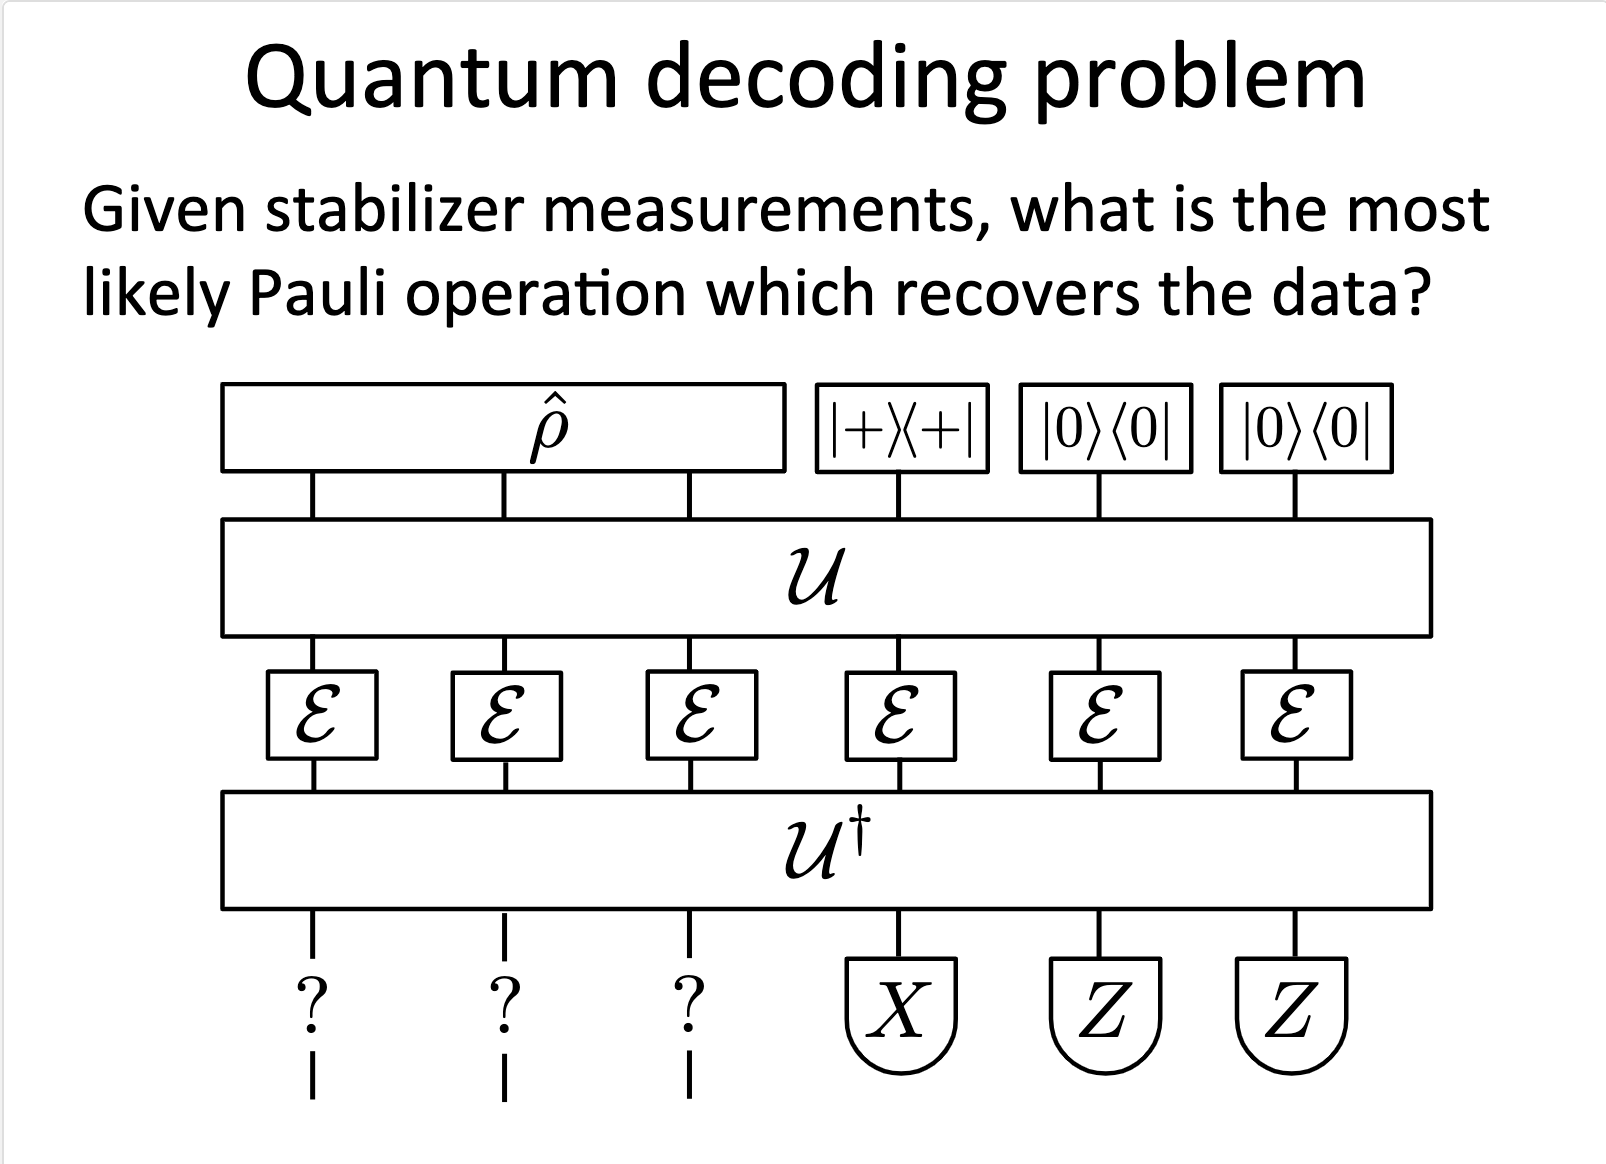
\includegraphics[scale=0.3]{../assets/decoding_gate_picture.png}
    \caption{Gate Picture of the Decoding problem. \textcolor{BrickRed}{What are the stabilizers in this picture?}}
    \label{fig:decode-gate-picture}
\end{figure}

In Fig. \ref{fig:decode-gate-picture}, you have tensor networks picture of the following process described in the equation below.
\begin{equation*}
    \rho \rightarrow Encode \rightarrow Error \rightarrow De-Encode \rightarrow Measure/Decode
\end{equation*}

\begin{figure}[ht]
    \centering
    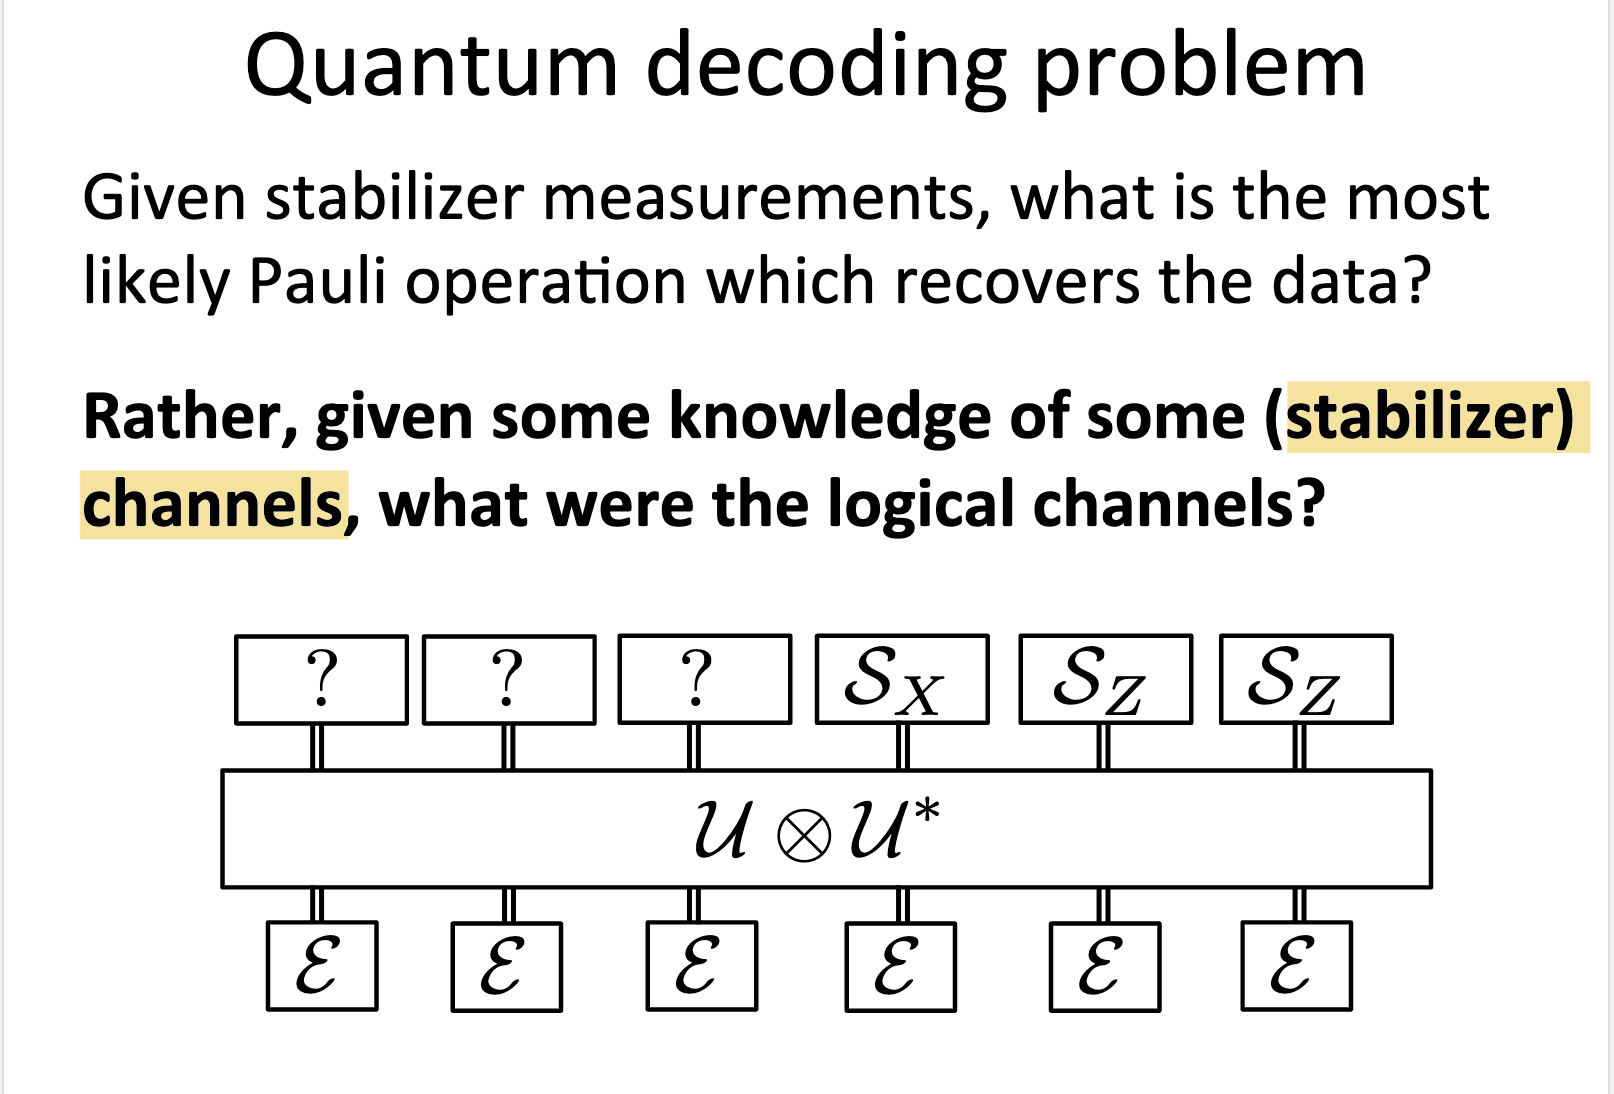
\includegraphics[scale=0.3]{../assets/decoding_channel_picture.png}
    \caption{Channel Picture of the Decoding problem. \textcolor{BrickRed}{What are the stabilizers in this picture?}}
    \label{fig:decode-channel-picture}
\end{figure}


\begin{quote}
    Thoughts from Alex Müller Hermes. For the Pauli Channel picture, Poulin is probably using one of the following. 
    \begin{align*}
        \rho \rightarrow \sum_{i = {0,1 2,3}} p_i Tr(\sigma_i \rho) \\
        \rho \rightarrow \sum_{i = {0,1 2,3}} p_i  \sigma_i \rho \sigma_i  \\
    \end{align*}
    In the end, this makes sense, because he is just re-orderding the tensor network in a different way. He did say something along the lines of prepare and measure $\ket{0}$.
\end{quote}

\textbf{How does $e = (1,1,1,1)$ correspond to the partial trace operations?}
\begin{itemize}
    \item If I just do it for single qubit line, it should correspond to the trace operation. Maybe this condition does not make sense.(Why?)
    \item If I do it for a bell pair, the partical trace should give me a maximally mixed state.
\end{itemize}

How to write the partial trace operation in the operator basis. What you get out in the end is the coefficient for the matrices $\{I, X, Y, Z\}$
Doing it in a single qubit line, given a state, in the form a density matrix $\rho$. Is there a requirment to choose a basis when performing the trace?

\begin{align*}
    \text{Trace} \equiv 
\end{align*}

Say I have single qubit density matrix $\rho$, which is a $rank-2$ tensor. What does $Tr(\sigma_j \rho)$ give me? It gives the expectation value of the measurement along the $\sigma_j$ axis of the qubit. Since ${\sigma_j}$ form a basis for the operator space of single qubit operations, any single qubit transformation can be characterized by 


\textbf{How does $b_z =(1,0,0,1)$ and $\bar{b_z} = (0,1,1,0)$ correspond to syndromes 0 and 1 respectively?}
One construct $b_z$ by the measure and prepare hypothesis. This being, if you prepare it in one of the eigenstate of the measurement basis, then it stays in the same eigenstate when there is no error. The nomenclature Quantum Stabilizer Channels makes no sense as it's a misnomer and can lead to the reader thinking this channel auto reverts from the onset of an error to one of the stabilizer states. 



\section{On indicator functions}
In appendix A of DP 2017, the author provide a presricption for representing a channel using a $4 \times 4$ process matrix. This section tries to reason how one may arrive at the indicator functions taking advantage of the channel-state duality offered by the Choi-Jamiolkowski Isomorphism. Ferris, in his talk on Tensor Networks and Quantum Error Correction, reposed the decoding channel in terms of channels. In partcular, he has asks: Given knowledge of some stabilizer channels, what the logical channel of the data qubits or the logical channel of the logical qubits. Poulin's reuses this framework in Tensor Networks Simulations of the Surface Code, in his 2017 paper Darmawan. 


Biamonte in his lectures on Quantum Tensor Networks, shows how to model the Choi Jamilowski Isomorphism as Tensor Network, adding an extra index for each qubit. 


\section{Notes on Christmas}

The ideas to evaluate until the next meeting.
\begin{enumerate}
    \item MPS decoding with noisy measurement
    \item write the introduction section of the thesis, with defining the stablizer, quantum codes and formal introduction to the decoding problem
    \item Subsection defining approximate decoding, minimum weight decoding and max likelihood decoding. 
    \item Definitions of thresholds and pseudothresholds
    \item thesis section on Tensor network representation of the toric code as the exemplar problem
    \item Thesis section of group and cosets.
    \item Proof on the equivalence between decoding concatenated quantum codes using tensor networks and it's equivalence to Belief propogation
    \item Basic thoughts on the ideas of Entanglement phases with weak measurements as to study quantum codes with tensor networks (see the latest set of papers on entanglement phases)
    \item Understand entanglement phase characterization through the concept of entanglement phase transisitions
    \item Classical Spin Models as the bridge for interconversion between different tensor network ansatze
    \item Understand the tensor network decoder of the Darmawan where they using logic representation of this problem
    \item analyse the list of CSS Codes examples provided by Niko Breuckmann
    \item Clearly understand the partition functions of the Ising Model 
    \item Understand the difference between order parameters and disorder parameters
    \item Does the rate of measurements define the transition between MBQC, CBQC and FBQC?s
    \item If Flag Gadgets can be constructed using Classical Codes and classical codes can be decoded using Tensor Network methods, then the Quantum Legos framework can be extended to include flag fault tolerant error correction methods?
\end{enumerate}

\subsection{Elucidating the thought experiments in Monitored Quantum Circuits}
There is a huge literature of papers for classfifying entangelment phases through monitored quantum circuits. Monitored Quantum Circuits, are circuits with mid-circuit measurements as a feature. A simple test is the study of entanglement dynamics in Lattice Surgery merge and split operations as a simple test. I hypothesisze I should be able to relate this to the stability experiments of Craig Gidney. Need to understand the difference between Entanglement Dynamics and Information Dynamics. Are weak measurements the same as ancilla assisted projective measurments? It looks like yes is the answer. 

What is the goal, we want to model noisy measurments of the stabilizer checks? In particular, if flag gadgets form a part of monitored quantum circuits. The paper on Nishimori's cat makes a relation between the weak measurement protocols, it's TN representation and Nishimori Physics. The Nishimori cat paper describes the Multibody Measurement via an ancilla. One way to study the lifetimes of the merge and the split protocols. 


Weak Monitoring - Applying a strong projective measurement on a qubit with probability \(p\)
Weak Measurements - strong projective measurement of weakly coupled ancilla qubit.
Does weak monitoring and weak measurements represent the same dynamics effectively?


\section{Measurement Phases, Entanglement Phases and QEC Phases}
All of these phases are different and this difference brought simply for the (dis)order parameter. \textbf{TODO} Identify the order and disorder parameters in these different cases and formulate a hypothesis to related to the decoding problem. MWPM, Max Likelihood decoding lie along different points of the Nishimori line.



\section{On Tensor Network Decoding and Belief Propogation Decoding of concatenated Quantum Codes}
\textit{The hypothesis}: We want to prove belief propogation contraction of tensor networks for the decoding the quantum error correcting code is the same as the belief propogation decoding of concatenated quantum codes(David Poulin). I think Tensor Network Codes already proves this through example construction of a concatenated code. It kind of looks trivial, Poulin's exact decoder is the same as the efficient contraction stragetry. Concatentation produces a tree and the efficient contraction goes from the leaf to the root. Poulin's similarly suggest decoding from the last block of concatenation towards the first level of concatenation, conditioned on the syndrome. The only thing that is not obvious is how the conditioning of the syndrome takes in Faralley's construction.



\section{On the Plurality of Tensor Network Represenation of QEC Codes}
That there exists "good" tensor network constructions of QEC codes is not suprising. After all, tensor networks were designed to efficiently simulate quantum systems. Since QM is linear, TN can effectively represent any linear system. On way of introducing non-linearity into tensor networks is through the framework of weak measurements. Holographic, concatenated and convolutional codes have a "good" TN representation. By "good" TN, we mean that it can be efficiently and exactly contracted. 

\textbf{Questions}
\begin{enumerate}
    \item Do a lit review on the classification of TN contraction problems. 
    \item Do convolutional codes have a "good" TN representation?
    \item The Toric Code has representation as a MERA, PEPS and MPS. Can the plurality be extended to other codes also? One thing to investigate here is the different representation efficent for a particular spatio-temportal correlation of the underlying noise model the syndromes are sampled from?
    \item One thing I do not understand at all is the mapping to Fermionic Gaussian States. 
    \item How does this plurality manifest? What I am asking is, if each representation represents a node on a graph and the presence of an edge indicating the presence of a duality between these two representations, what kind of network do I have?
\end{enumerate}
\end{document}